\section{Single cooper pair box system\label{sec:cooper_pair_box}}
The Cooper pairs are trapped on an island between a gated capacitor and a Josephson junction.
\begin{figure}[h]
  \centering 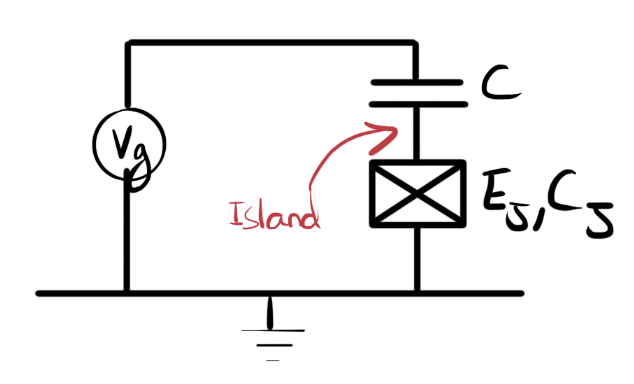
\includegraphics[height=4cm]{cooper_pair_box}
\end{figure}

\noindent

\begin{framed}\noindent
  We remember that the voltage induction law reads
  \begin{equation}\label{key}
    V = -\dot{\Phi}.
  \end{equation}
\end{framed}


\begin{enumerate}
\item Forgetting about  the voltage source, we consider  the following diagram, which will  have a \red{\textbf{charging
      kinetic part}}

  \begin{equation}\label{key}
    T = \frac{C_g}{2}\dot{\Phi_J}^2 + \frac{C_J}{2}\dot{\Phi_J}^2 = \frac{C_\Sigma}{2}\dot{\Phi_J}^2.
  \end{equation}

\begin{figure}[h]
  \centering 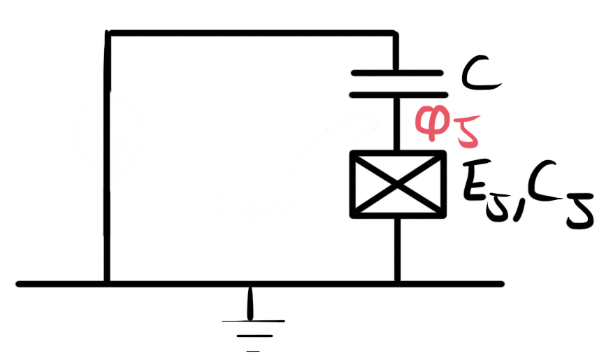
\includegraphics[height=3cm]{cooper_pair_box_1}
\end{figure}

\noindent

\item \textbf{\red{The potential  energy part}} comes from the JJs  and the energy supplied by the  source acting on the
  gate side of the gate capacitor (note that we are free to choose the sign of the biasing voltage.
  \begin{equation}\label{key}
    \begin{aligned}
      & E_J = 1 - E_J\cos(\frac{2\pi}{\Phi_0}\Phi_J)\\
      & \begin{aligned}
        E_\text{gate} & = V_g \times Q_c\\
        Q_c & = C_g\times -\dot{\Phi_J}
      \end{aligned}
    \end{aligned}\ira U = -E_J\cos(\frac{2\pi}{\Phi_0}\Phi_J) - V_gC_g\dot{\Phi_J}.
  \end{equation}

\begin{figure}[h]
  \centering 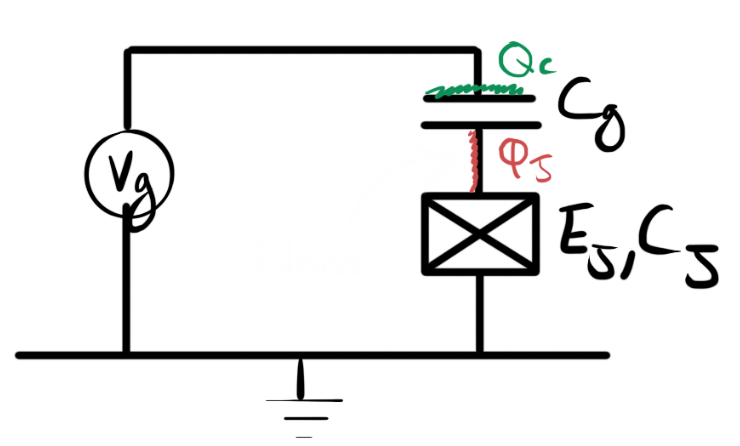
\includegraphics[height=3cm]{cooper_pair_box_2}
\end{figure}

\noindent

\item The full \red{\textbf{Lagrangian}} now reads
  \begin{equation}\label{key}
    \mathcal{L} = T - U = \frac{C_\Sigma}{2}\dot{\Phi}_J^2 + E_J\cos(\frac{2\pi}{\Phi_0}\Phi_J) + V_gC_g\dot{\Phi_J}.
  \end{equation}

\item The \textbf{\red{conjugate momentum}}
  \begin{equation}\label{key}
    Q_J = \frac{d\mathcal{L}}{d\dot{\Phi}_J} = C_\Sigma\dot{\Phi}_J + V_gC_g,
  \end{equation}
  \noindent is just an offset of the induced charge on the capacitor due to the JJ voltage with the gate induced charge.

\item So we arrive at the following set of variables

  \begin{equation}
    { \textcolor{blue}{\mathbf{x\leftrightarrow \Phi \leftrightarrow \phi} \text{ (position/flux) }}\qquad \textcolor{red}{\mathbf{p\leftrightarrow Q \leftrightarrow N \text{ (momentum/electrons) }}}}
  \end{equation}

  \noindent with the commutation relations:

  \begin{align}
    \left[\blue{x},\red{p}\right] & =i\hbar & \left[\blue{\Phi},\red{Q}\right] & = i\hbar & \left[\phi,N\right] & = \frac{2\pi}{\frac{h}{2e}}\left[\Phi,Q\right]\frac{1}{2e} = i\\
    \red{\hat{p}} & = -i\hbar\ipartial{}{\blue{x}} & \hat{\red{Q}} & =-i\hbar\ipartial{}{\blue{\Phi}} & \hat{\red{N}} & =-i\ipartial{}{\blue{\phi}}
  \end{align}

\item\

\begin{framed}\noindent
  Expressing the \red{\textbf{Hamiltonian}} in the standard fashion

  \begin{equation}\label{eqn:cpbox_final}
    \begin{aligned}
      \mathcal{H} & = Q_J\dot{\Phi}_J - \mathcal{L}\\
      & = \frac{(Q_J - C_gV_g)^2}{2C_\Sigma} - E_J\cos(\frac{2\pi}{\Phi_0}\Phi_J)\\
      &     =      \mathbf{\red{E_C{\left(\hat{N}-N_\text{ext}\right)^2}-     E_J\cos\left(\phi\right)}}\qquad      E_c     =
      \frac{(2e)^2}{2C_\Sigma}
    \end{aligned}
  \end{equation}

  \noindent Wel call $ N_\text{ext} = \frac{C_\Sigma V_g}{2e} $ the effective offset charge.
\end{framed}
\end{enumerate}

\subsection{Adding a parallel JJ\label{subsec:cpb_2}}
\begin{figure}[h]
  \centering 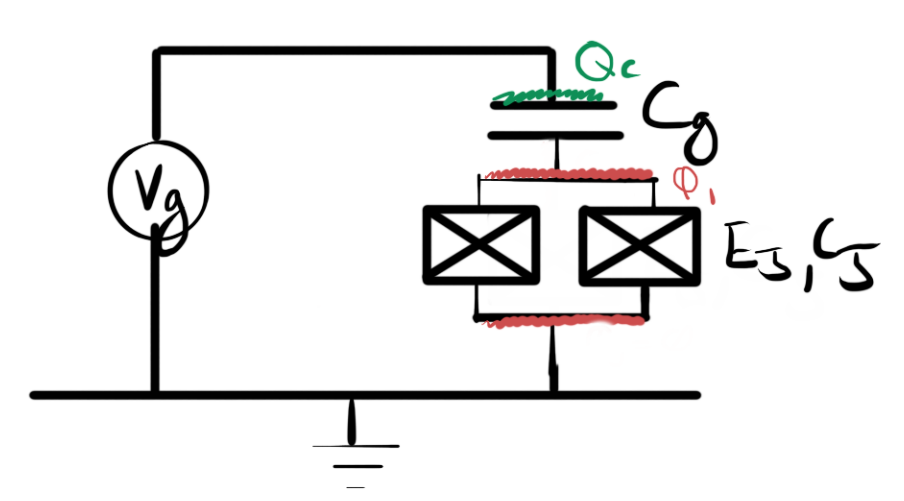
\includegraphics[height=5cm]{cooper_pair_box_4}
\end{figure}

\noindent
Adding a second JJ in parallel, will allow us to control the Josephson energy $ E_J $.
\begin{itemize}
\item    The   two    currents   throught    the   JJ    wil    give   a    total   current    \begin{equation}   I    =
    I_{c1}\sin(\phi_1)+I_{c2}\sin(\phi_2),
  \end{equation}

\item Along with the phase quantisation $ \phi_1+\phi_2+\phi_\text{ext} = 2\pi m $ and symmetric JJs $I_{c1}=I_{c2}=I_c$
  results in

  \begin{equation}
    \begin{aligned}
      I & = 2I_c\sin(\frac{\phi_1+\phi_2}{2})\cos(\frac{\phi_1-\phi_2}{2})) \\
    \end{aligned}
  \end{equation}

\begin{framed}\noindent
  Or in more general form
  \begin{equation}\label{key}
    I = I_{cs}\sin(\phi)
  \end{equation}
  \noindent where
  \begin{equation}\label{key}
    I_{cs} = 2I_c|\cos(\pi\Phi_\text{ext}/\Phi_0)|\qquad \phi = (\phi_1+\phi_2)/2
  \end{equation}

\end{framed}

\item The Josephson energy

  \begin{equation}
    \left\lbrace\begin{aligned}
        I &= I_{cs}\sin(\phi)\\
        V&=\dot{\Phi} \equiv \frac{\dot{\phi}}{2\pi}\Phi_0
      \end{aligned}\right. \Rightarrow U = \left\lbrace\begin{aligned}
        \int_{0}^{t}IV dt & = \int_{0}^{t}I_{cs}\sin(\phi)\frac{\Phi_0}{2\pi}\frac{d\phi}{dt}dt\\
        & = \int_{0}^{\phi} E_{Js}\sin(\phi)d\phi\\
        & \red{= E_{Js}(1-\cos(\phi)),\qquad E_{Js} = \frac{\Phi_0I_c}{2\pi}\times 2|\cos(\pi\Phi_\text{ext}/\Phi_0)|.}
      \end{aligned}\right.
  \end{equation}
  \begin{framed}\noindent
    \textbf{Acquires an additional factor which can now be controlled
      \begin{equation}\label{key}
        2|\cos(\pi\Phi_\text{ext}/\Phi_0)|
      \end{equation}}
  \end{framed}
\end{itemize}

\subsection{Quantising the Hamiltonian}
\subsubsection{\red{Charge energy dominates}, $ E_C/E_J >> 1$}
If charge is  the important variable, then we  chall work with the  charge basis $ \lbrace N  \rbrace $. We use the  number of phase
operators derived in App.~\ref{sec:charge_basis}

\begin{framed}\noindent

  \begin{equation}\label{key}
    \begin{aligned}
      e^{\pm i\hat{\blue{\phi}}} & = \sum_{n}\iketbra{n\pm 1}{n}\\
      \hat{\red{N}} & = \sum_{n}n\iketbra{n}{n}.
    \end{aligned}
  \end{equation}

\end{framed}

\noindent and using the exponential form of cos, we rewrite Eq.\eqref{eqn:cpbox_final}

\begin{equation}
  \begin{aligned}
    \mathcal{H} & = E_C{\left(\hat{\red{N}}-N_\text{ext}\right)^2}- E_J\cos\left(\hat{\blue{\phi}}\right)\\
    & = \sum_n\bigg[E_C{\left(n-N_\text{ext}\right)^2}\iketbra{n}{n}- \frac{E_J}{2}\bigg(\iketbra{n+1}{n}+\iketbra{n-1}{n}\bigg)\bigg]\\
    & = \begin{pmatrix}
      E_C(-2-N_\text{ext})^2 & -E_J/2 & 0 & 0 & 0\\
      -E_J/2 & \red{E_C(-1-N_\text{ext})^2} & \red{-E_J/2} & 0 & 0\\
      0 & \red{-E_J/2} & \red{E_C(N_\text{ext})^2} & -E_J/2 & 0\\
      0 & 0 & -E_J/2 & E_C(1-N_\text{ext})^2 & -E_J/2\\
      0 & 0& 0 & -E_J/2 & E_C(2-N_\text{ext})^2\\
    \end{pmatrix}
  \end{aligned}.
  \label{l2-subbed2}
\end{equation}

\begin{figure}[h]
  \centering 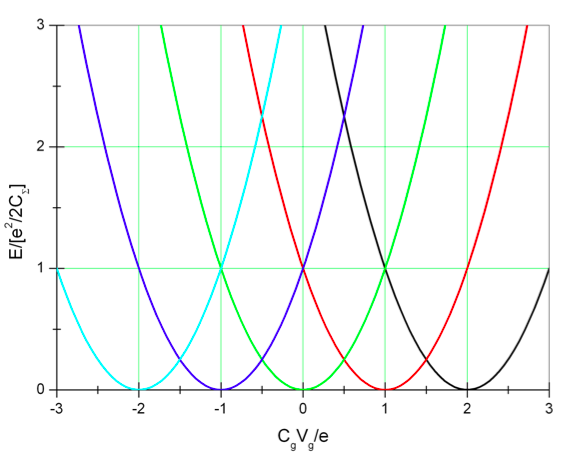
\includegraphics[height=3cm]{island}
  \caption{\small  System will  be  in the  lowest  energy  state, i.e.   have  that many  electrons  that minimize  its
    energy\label{fig:cp_box_energy_charge}}
\end{figure}

\noindent

\noindent Normally  $ N_\text{ext}  $ is  biased at a  sweet spot  \red{close to  $ - 1/2  $}. Then  the only  number of
electrons   $n$   on   out   island   that   will   give   a   low   energy   (due   to   the   energy   dispersion   in
Fig.~\ref{fig:cp_box_energy_charge}) is either  0 or -1.  The  other level will be  far separated. Then we  take out the
Hamiltonian

\red{\begin{equation}
    \begin{aligned}
      \mathcal{H}_\text{0 or -1} & = \begin{pmatrix}
        E_C(-1-N_\text{ext})^2 & -E_J/2\\
        -E_J/2 & E_C(N_\text{ext})^2\\
      \end{pmatrix}\\
    \end{aligned}
  \end{equation}}

\noindent  And  we  have  a  two  level  system  just as  in  the  previous  lecture  Eq.\eqref{l1-finalEVal}  shown  in
Fig.\ref{l2-closeup}. Redefining the zero point energy to be in the middle of the diagonal terms

\begin{equation}
  \begin{aligned}
    \mathcal{H} & = \begin{pmatrix}
      -\epsilon/2 & -E_J/2\\
      -E_J/2 & \epsilon/2\\
    \end{pmatrix}\\
    \epsilon/2    =   \frac{\text{energy    diff}}{2}    &    =   \frac{E_CN_\text{ext}^2-E_C(1+N_\text{ext})^2}{2}    =
    -\frac{E_C}{2}\big(1+2N_\text{ext}\big)
  \end{aligned}
\end{equation}

\begin{framed}\noindent
  This will have solutions

   \begin{equation}
     E = \pm \frac{\Delta E}{2}, \qquad \ket{\psi}_0 = \begin{pmatrix}
       \cos(\theta/2) \\ \sin(\theta/2)
     \end{pmatrix}, \qquad \ket{\psi}_1 = \begin{pmatrix} \sin(\theta/2) \\ \cos(\theta/2)
     \end{pmatrix}, \Delta E = \sqrt{\epsilon^2+\Delta^2}
   \end{equation}
 \end{framed}

 \begin{itemize}
 \item In  Fig.\ref{l3-energyspec} depicted  are the energy  levels for  different values of  the charging  and coupling
   energies. The stronger the coupling, $ E_J $, the bigger the splitting at the degeneracy points.

   \red{There is less charge noise in  the sweet spots of $ n_g = \mathbb{Z}\frac{1}{2} $, but  it will still be a major
     source of decoherence. \textbf{There is less dependence on charge  fluctuations as $ E_C/E_J $ gets smaller and the
       band become flatter}.}
   \begin{figure}[h]
     \centering 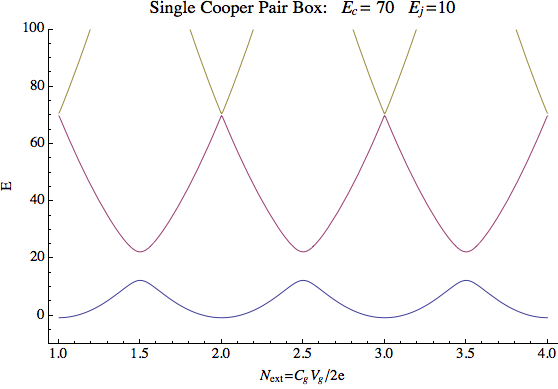
\includegraphics[height=6cm]{cpb2}
   \end{figure}

\noindent
different at the degeneracy point grows as coupling becomes stronger.\label{l3-energyspec}

\item One can also looks the ground energy state (the  one the system will most probably occupy) and find the components
  that make it up

  \[
    \Ket{\Psi}_{\text{ground}} = \sum_N\alpha_N\ket{N},
  \]

  \noindent and one sees in the  figures when there is no applied gate voltage, the island will  have $ N=0 $ charges on
  it predominantly. As one increases the gate charge, the presence of $ N=1 $ increases, until it finally dominates. The
  pattern repeats as more and more cooper pairs tunnel, to give the lowest energy configuration.

\begin{figure}[h]
  \centering 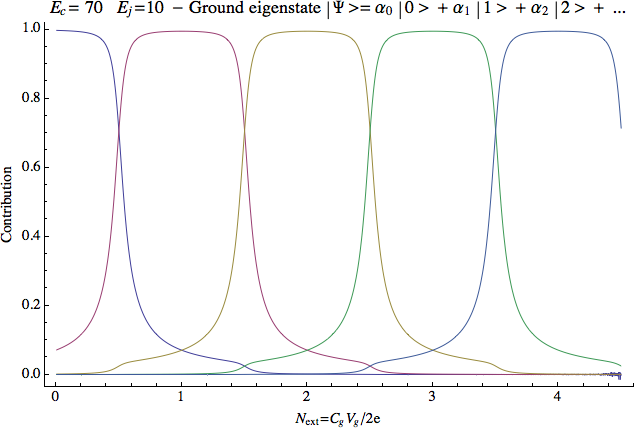
\includegraphics[height=5cm]{cpb3}
\end{figure}

\noindent
\begin{figure}[h]
  \centering 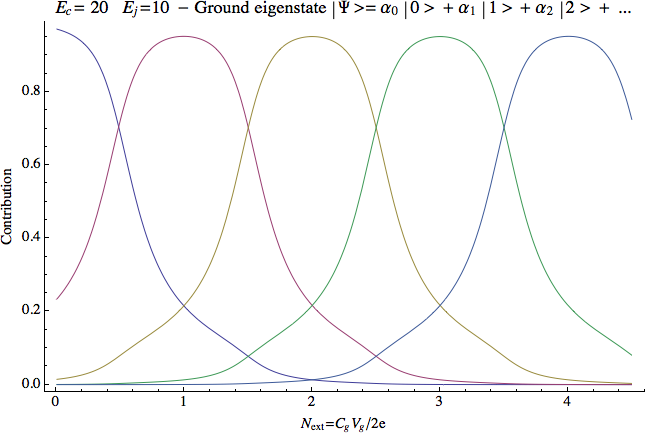
\includegraphics[height=5cm]{cpb4}
\end{figure}

\noindent

\end{itemize}

\begin{framed}\noindent
  \textbf{High $ E_C/E_J $:}
  \begin{itemize}
  \item High charge noise - gate voltage changes, affects the energy levels severely
  \item High anharmonicity - quadratic $ n $ dependance dominates, allowing individual addressing of the levels;
  \end{itemize}

\end{framed}

\newpage\subsubsection{\red{Flux energy dominates, $ E_C/E_J << 1 $}}
If flux is the important variable, then we chall work with the flux basis using the wavefunctions $ \psi(\phi) $

\begin{framed}\noindent

  \begin{equation}\label{key}
    \begin{aligned}
      &\blue{\hat{\phi}} \qquad\\
      &\red{\hat{N}} = -i\frac{d}{d\blue{\phi}}
    \end{aligned}
  \end{equation}

\end{framed}
\noindent and we rewrite

\begin{equation}\label{key}
  \begin{aligned}
    \mathcal{H} & = E_C{\left(\hat{\red{N}}-N_\text{ext}\right)^2}- E_J\cos\left(\hat{\blue{\phi}}\right)\\
    & = E_C\left(-i\frac{d}{d\phi} - n_g\right)^2 - E_J\cos(\phi).
  \end{aligned}
\end{equation}

\begin{itemize}
\item Let us compare this to Hamiltonian in a periodic potential
  \begin{equation}\label{key}
    \mathcal{H}_\text{crystal} = \frac{-\hbar^2}{2m}\frac{d^2}{dx^2}+V(x)\qquad V(x+a) = V(x),
  \end{equation}

  \noindent which, according to Bloch's theorem, states that the eigenstates will be of the form
  \begin{equation}\label{key}
    \psi_{kn}(x) = e^{ikx}u_{kn}(x),
  \end{equation}
  \noindent which, when plugged in will result in an effective Hamiltonian

  \begin{equation}\label{key}
    \mathcal{H}_{\text{eff},k} = \frac{\hbar^2}{2m}\left(-i\frac{d}{dx}+k\right)^2 + V(x)
  \end{equation}
\item We can see this mapping between
  \begin{equation}\label{key}
    \begin{aligned}
      \mathcal{H}_{\text{eff},k} & = \frac{\hbar^2}{2m}\left(-i\frac{d}{dx}+k\right)^2 + V(x)\\
      \mathcal{H} & = E_C\left(-i\frac{d}{d\phi} - n_g\right)^2 - E_J\cos(\phi),
    \end{aligned}
  \end{equation}

  \noindent so, will look for solutions of a similar form.
\item As $ E_C/E_J  $ gets smaller, the potential well  from the $ E_J\cos(\phi) $ gets  deeper \red{\textbf{and the states
      within each well localise, and  stop interacting with one another.}} Solving, as in  the Transmon Paper, will lead
  to anharmonicity relation

  \begin{framed}\noindent
    \begin{equation}\label{key} \frac{E_{12} - E_{01}}{E_{01}}\approx -(8E_J/E_C)^{-1/2},
    \end{equation}
    \noindent which decreases as we continue to increase $ E_J $.
  \end{framed}
\end{itemize}
\newpage
